% AIR — Auto-Interpretability Router: protocol overview figure.
% Standalone TikZ. Compile:  pdflatex protocol_overview.tex
% Include in paper:          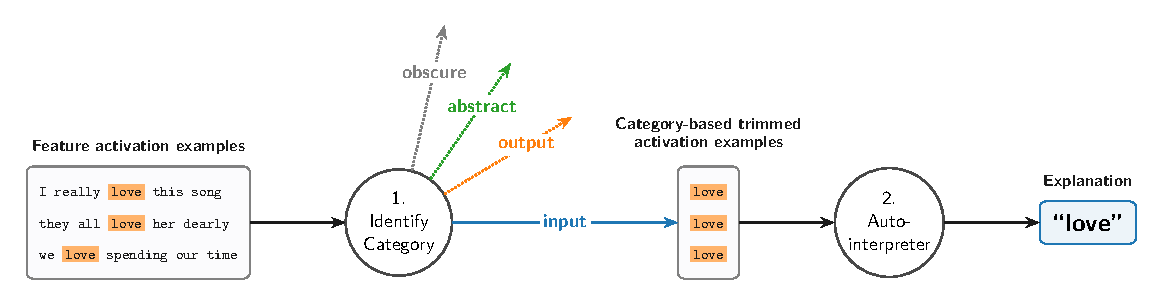
\includegraphics{protocol_overview.pdf}
\documentclass[border=12pt]{standalone}
\usepackage{lmodern}
\usepackage{xcolor}
\usepackage{tikz}
\usetikzlibrary{positioning, arrows.meta, calc}

% Palette matches CATEGORY_COLORS (matplotlib tab colors) used elsewhere in the project.
\definecolor{inputc}{HTML}{1F77B4}
\definecolor{outputc}{HTML}{FF7F0E}
\definecolor{abstractc}{HTML}{2CA02C}
\definecolor{obscurec}{HTML}{7F7F7F}
\definecolor{hl}{HTML}{FFB36B}      % activation highlight
\definecolor{ink}{HTML}{1A1A1A}
\definecolor{panel}{HTML}{FBFBFD}

\setlength{\fboxsep}{1.4pt}
\newcommand{\tok}[1]{\colorbox{hl}{\textbf{#1}}}   % max-activation token

\begin{document}
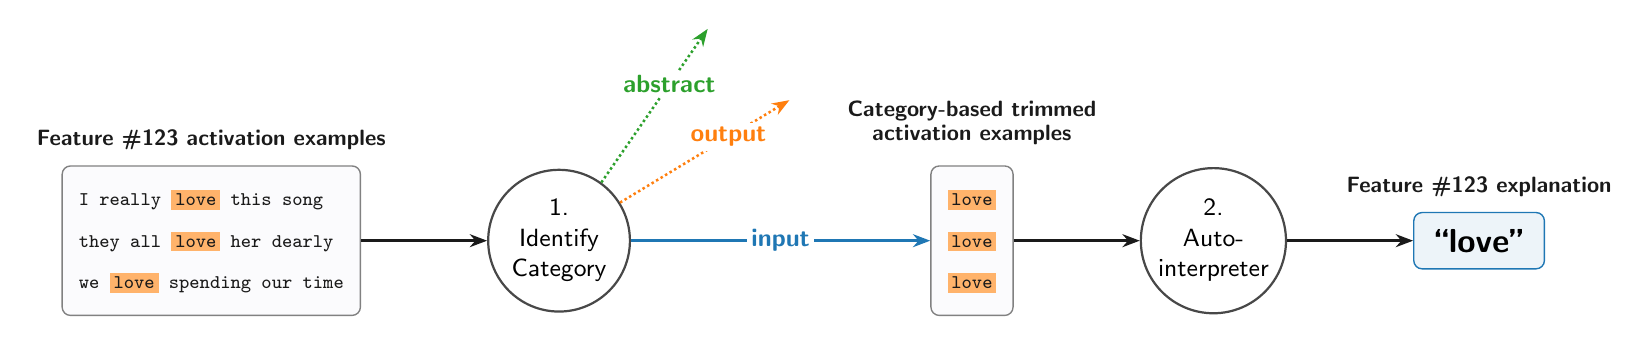
\begin{tikzpicture}[
  font=\sffamily,
  >={Stealth[length=2.2mm]},
  box/.style={rounded corners=3pt, draw=ink!55, line width=0.5pt, fill=panel, inner sep=6pt, align=left},
  title/.style={font=\sffamily\bfseries\footnotesize, text=ink},
  fn/.style={circle, draw=ink!80, line width=0.8pt, fill=white, align=center,
             font=\sffamily\small, minimum size=18mm, inner sep=1pt},
  route/.style={font=\sffamily\bfseries\small, fill=white, inner sep=1.5pt},
  arr/.style={->, line width=0.9pt, draw=ink},
  darr/.style={->, line width=0.9pt, densely dotted},
]
\newcommand{\ex}[1]{{\ttfamily\scriptsize\color{ink}#1}}

% ---------------- Feature (left) ----------------
\node[box] (feat) {%
  \begin{tabular}{@{}l@{}}
  \ex{I really \tok{love} this song}\\[3pt]
  \ex{they all \tok{love} her dearly}\\[3pt]
  \ex{we \tok{love} spending our time}\\
  \end{tabular}};
\node[title, above=2pt of feat] {Feature \#123 activation examples};

% ---------------- 1. Identify Category ----------------
\node[fn, right=16mm of feat] (router) {1.\\Identify\\Category};
\draw[arr] (feat.east) -- (router.west);

% ---------------- routing fan (4 labelled arrows) ----------------
% input is solid and continues the pipeline; the others are dotted alternatives.
\draw[darr, outputc]   (router.32) -- ++(2.15,1.30) node[route, text=outputc,   pos=0.64]{output};
\draw[darr, abstractc] (router.54) -- ++(1.35,1.95) node[route, text=abstractc, pos=0.64]{abstract};
%\draw[darr, obscurec]  (router.76) -- ++(0.55,2.45) node[route, text=obscurec,  pos=0.68]{obscure};

% ---------------- Trimmed examples (input route) ----------------
\node[box, right=38mm of router] (trim) {%
  \begin{tabular}{@{}l@{}}
  \ex{\tok{love}}\\[3pt]
  \ex{\tok{love}}\\[3pt]
  \ex{\tok{love}}\\
  \end{tabular}};
\node[title, above=4pt of trim, align=center] {Category-based trimmed\\[-1pt]activation examples};
\draw[arr, inputc] (router.east) -- (trim.west) node[route, text=inputc, midway]{input};

% ---------------- 2. Auto-interpreter ----------------
\node[fn, right=16mm of trim] (interp) {2.\\Auto-\\interpreter};
\draw[arr] (trim.east) -- (interp.west);

% ---------------- Explanation (output) ----------------
\node[box, draw=inputc, fill=inputc!8, right=16mm of interp] (expl) {\large\bfseries ``love''};
\node[title, above=2pt of expl] {Feature \#123 explanation};
\draw[arr] (interp.east) -- (expl.west);

\end{tikzpicture}
\end{document}
